\section{Repeated games, grim trigger, tit for tat, Friedman theorem}

\Que{What is a repeated game?}
\Ans[A repeated game $\ml{G}(T, \delta)$]{ is a dynamic game where a static game $\ml{G}$ is played as a stage game for $t$ times with discount $\delta$. We distinguish between:
\begin{itemize}
    \item finitely repeated games ($T = 1, 2, \dots < \infty$);
    \item infinitely repeated games ($T = \infty$). Here we must have $\delta < 1$, otherwise payoff will diverge.
\end{itemize}}

\Que{Theorems}
\Ans[]{
\begin{enumerate}
    \item The outcome of the last stage is a NE
    \item If stage game $\ml{G}$ only has NE $p^*$, then $\ml{G}(T, \delta)$ has a unique subgame-perfect equilibrium, where every player play $p^*$ in every stage (boring)
\end{enumerate}
}

\Que{Cooperation in finitely repeated games}
\Ans[Cooperation ]{is usually incentived in repeated games but in the last stage, which is played "egoistically". As for multistage games, cooperation is possible if there are multiple NE.}

\Que{Infinitely repeated game}
\Ans[]{Since these games has no last stage, there could be a SPE of $\ml{G}(\infty, \delta)$ in which no stage outcome is a NE of $\ml{G}$.

We call a \textbf{grim trigger strategy} (GrT) a strategy where: start playing M at stage 1, at stage $t > 1$, play M only if outcome of all $t-1$ previous stages was $(M,m)$, otherwise play F.\\With $\delta = 1 - \epsilon$, joint strategy "both play GrT" is a SPE.}

\Que{How can we show that a strategy is a NE in overall game?}
\Ans[]{We only need to compare who options:
\begin{itemize}
    \item Cooperate and keep playing the chosen strategy (payoff $^*$) forever (\m{u_T = p^* + \delta p^* + \delta^2 p^* + \dots = \frac{p^*}{1-\delta}})
    \item Defect at stage 1 and keep playing other option (payoff $p$) forever (\m{u_T = p + \delta p + \delta^2 p + \dots = p + \frac{\delta}{1-\delta}})
\end{itemize}
In order to fine minimum $\delta$ s.t. cooperation is best choice, solve \mat{\frac{p^*}{1-\delta} \geq p + \frac{\delta}{1-\delta}}
}

\Que{Friedman theorem (a.k.a. "folk theorem")}
\Ans[Theorem]{ Let $\ml{G}$ be a finite static game of complete information. Let $(e_1, e_2, \dots, e_n)$ be the payoffs of a NE of $\ml{G}$ and $(x_1, x_2, \dots, x_n)$ be a feasible payoffs for $\ml{G}$. Suppose $\fa$ NE and $\fa, x_j > e_j$. Then, for $\delta$ close enough to 1, $\ml{G}(\infty, \delta)$ has a SPE with payoffs $(x_1, x_2, \dots, x_j)$.
\begin{figure}[!ht]
    \centering
    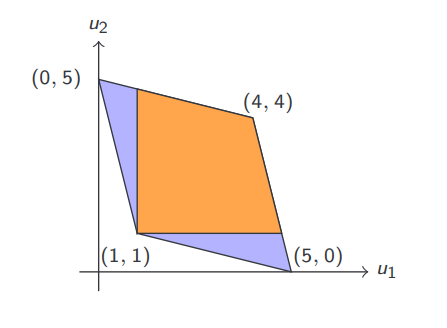
\includegraphics[width=0.3\linewidth]{Friedman.png}
\end{figure}
}
\Spec{A \textbf{feasible payoff} for game $\ml{G}$ is any convex combination \mat{\alpha u(s_1) + \alpha u(s_2) + \dots + \alpha_L(s_L), \text{with} \sum_{i=1}^L\alpha_i=1} of pure-strategy payoffs ($L = |S_1| \cdot |S_2| \dotsm |S_n|$ total numbers of pure strategy)
\begin{figure}[!ht]
    \centering
    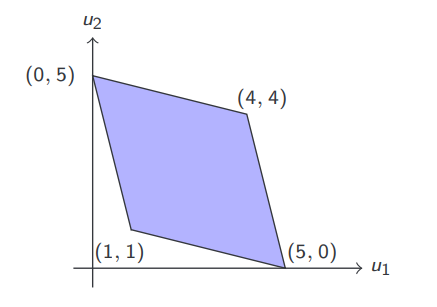
\includegraphics[width=0.3\linewidth]{feasiblePayoff.png}
\end{figure}
}

\Que{Tit for tat (TFT)}
\Ans[TFT ]{is a replacement of GrT where "at stage $t$, play what the other player chose at stage $t-1$", it's a way to avoid keep punishment forever. It has immediately punish deviation but forgiveness after 1-step.

Keep doing TFT forever is called "death spiral" and it's not a NE. generally, NE achieved by TFT is not subgame-perfect.}

\Que{Exercise 1

Consider $\ml{G}$:
\begin{table}[!ht]
\centering
\begin{tabular}{lccc}
& & \multicolumn{2}{c}{Player B} \\
\multirow{3}{*}{\rotatebox{90}{Player A}} & & g & w \\ \cline{3-4} 
& \multicolumn{1}{c|}{G} & \multicolumn{1}{c|}{5, 3} & \multicolumn{1}{c|}{0, 4} \\ \cline{3-4} 
& \multicolumn{1}{c|}{N} & \multicolumn{1}{c|}{6, 0} & \multicolumn{1}{c|}{1,1}  \\ \cline{3-4} 
\end{tabular}
\end{table}
\begin{enumerate}
    \item Is it possible to find a SPE for $\ml{G}$(4) that involves playing (G,g) at each stage?
    \item Is it possible to find a NE for $\ml{G}$($\infty$) where (G,g) is played at each stage using a grim-trigger strategy? If so, for what $\delta$? Is that a SPE?
    \item Is it possible to find a NE for $\ml{G}$($\infty$) where (G,g) is played at each stage using a tit-for-tat strategy? If so, for what $\delta$? Is that a SPE?
\end{enumerate}}
\Ans[]{
TODO:
}

\Que{Exercise 2

Carl (C) and Diana (D) are two university students. Every night they go to the department library, but they do not coordinate or plan any action together. Upon their arrival, they independently decide whether to: (S) study or (M) watch some movies on their laptop. If they both study, they both
get utility 10. The individual benefit from watching a movie is instead 15 for C and 18 for D. However, if they both choose M, their individual benefit is halved (since they have half the
connection speed). Also, trying studying while somebody else is playing a movie breaks the concentration, so $u_C(S,M) = u_D(M,S)$ = 0. Call $\ml{G}$ this game, and consider it in a repeated version $\ml{G}$(T). Individual payoffs are summed with discount factor $\delta$.
\begin{enumerate}
    \item Find the Nash equilibria of $\ml{G}$(3), for $\delta$ = 1
    \item What values of $\delta$ allow for sustaining a Nash equilibrium of $\ml{G}$($\infty$) via a “Grim Trigger” strategy where each player ends up in always choosing S?
    \item Consider an extended game where a punishment strategy P is also available to both players. When either player P, payoffs are -10 for both players (that would correspond, e.g., to do something really stupid in the library and get the library permanently closed). Call this game $\ml{G}$' . If you see a SPE of $\ml{G}$'(2) where players may play S, state at which round do they play it, and what value of $\delta$ do you need to obtain it.
\end{enumerate}}
\Ans[]{
TODO:
}